\subsection{Labelling engine lines, which is what the application actually does}\label{sec:nn-deployment}

Every number so far comes from puzzle solution lines. In the application the labeller sees something
else: Stockfish's principal variation from a critical position in a real game, cut to a fixed number
of plies. A puzzle solution stops when the tactic is complete; an engine line runs on into the won
position that follows. To measure that shift, 2{,}000 held-out harness puzzles were re-analysed with
the analyzer's own settings, and both labellers were scored on the engine line and on the solution
line of the same puzzles.

\begin{table}[H]
\centering
\small
\caption{Agreement with the Lichess category on 2{,}000 held-out puzzles, by the line the labeller is
shown. The engine's first move is the puzzle's first solution move in 99.3\% of these positions, so
the difference is about the line, not about the engine finding something else.}\label{tab:nn-engine}
\begin{tabularx}{\linewidth}{Xcc}
\toprule
\textbf{Line shown to the labeller} & \textbf{Strict agreement} & \textbf{$\kappa$} \\
\midrule
Rule-based tagger, puzzle solution        & 56.9\% & 0.504 \\
Rule-based tagger, engine line (7 plies)  & 55.5\% & 0.489 \\
\midrule
PuzzleNet, puzzle solution                & 91.9\% & 0.905 \\
PuzzleNet, engine line (1 ply)            & 66.4\% & 0.602 \\
PuzzleNet, engine line (3 plies)          & 80.3\% & 0.769 \\
\textbf{PuzzleNet, engine line (5 plies)} & \textbf{80.9\%} & \textbf{0.777} \\
PuzzleNet, engine line (7 plies)          & 76.5\% & 0.726 \\
\bottomrule
\end{tabularx}
\end{table}

\begin{honest}[Honest status: the network loses a third of its advantage in deployment]
PuzzleNet was trained on solution lines, so the engine line costs it a great deal: $\kappa$ falls from
0.91 to 0.78. The rule-based tagger barely moves (0.50 to 0.49), because it restricts which motifs may
be claimed at which depth and so ignores most of the continuation anyway. The deployed advantage is
therefore $\kappa = 0.78$ against $0.49$, not $0.91$ against $0.52$. It is still a large advantage,
and it is the honest one to quote for game analysis.
\end{honest}

The table also fixes a parameter. Agreement peaks when the network is shown five plies, and drops by
0.05 of $\kappa$ at seven, which is what the analyzer previously passed to the tagger. The deployed
system now gives the network the first five plies (\code{labeller.NEURAL\_PV\_PLIES}) and the
rule-based tagger the full line it was validated on. That is a measured choice, not a guess.

\subsection{What the network is actually learning: ablations}\label{sec:nn-ablations}

Every ablation trains on the same one-million-puzzle subset with the same schedule and is scored on
the same test split, so the rows differ only in what is named. The table is generated from
\code{eval/neural/puzzlenet\_evaluation.json} by \code{dissertation/build\_ablation\_table.py}, so it
cannot drift from the experiments.

\begin{table}[H]
\centering
\small
\caption{Ablations (1M training puzzles each) and the data-scaling sweep, all on the same test
split. $\kappa$ and macro-$F_1$ are the category head; RMSE is the difficulty head in rating points; a
dash means the model has no such head. Training times are not comparable across rows: the runs
shared a loaded laptop.}\label{tab:nn-ablations}
\begin{tabularx}{\linewidth}{Xcccc}
\toprule
\textbf{Variant} & \textbf{$\kappa$} & \textbf{Macro-$F_1$} & \textbf{RMSE} & \textbf{Train (s)} \\
\midrule
Reference: 512--256 trunk, all features, all heads & 0.867 & 0.774 & 285 & 516 \\
\midrule
No hidden layers (logistic / linear regression) & 0.743 & 0.610 & 326 & 294 \\
Raw boards and moves only & 0.741 & 0.645 & 313 & 505 \\
Hand-built relations only (no boards, no moves) & 0.830 & 0.708 & 305 & 74 \\
Wider trunk: 1024--512 & 0.878 & 0.797 & 280 & 4907 \\
\midrule
Category head alone (no multi-task) & 0.870 & 0.782 & --- & 486 \\
Difficulty head alone (no multi-task) & --- & --- & 280 & 468 \\
$\beta = 0$ (plain noise-aware likelihood) & 0.860 & 0.763 & 283 & 562 \\
$\beta = 1$ (squared-error gradient for the mean) & 0.868 & 0.777 & 289 & 250 \\
\midrule
30{,}000 training puzzles & 0.722 & 0.570 & 351 & 95 \\
100{,}000 & 0.780 & 0.654 & 333 & 127 \\
300{,}000 & 0.823 & 0.708 & 297 & 122 \\
1{,}000{,}000 & 0.867 & 0.774 & 285 & 516 \\
\textbf{5{,}526{,}626 (the production model)} & \textbf{0.914} & \textbf{0.861} & \textbf{268} & \textbf{2478} \\
\bottomrule
\end{tabularx}
\end{table}

\begin{finding}[Representation and data, not capacity]
The hand-built tactical relations carry most of the signal: on their own, with no boards and no move
blocks at all, they reach $\kappa = 0.830$ against $0.867$ for the full input. The raw boards and
moves on their own reach $0.741$. Each still adds something the other lacks --- the relations add
$0.126$ to the raw input, the raw input adds $0.037$ to the relations --- but a reader should not
conclude that the network has learned chess from squares. Depth matters about as much as the
relations: with no hidden layers, on the same features, $\kappa$ falls to $0.743$. Capacity is the
cheapest thing to buy and the least useful: four times the trunk buys $0.011$, while 5.5 times the
data buys $0.047$ and the curve has not flattened.
\end{finding}

\begin{figure}[H]
\centering
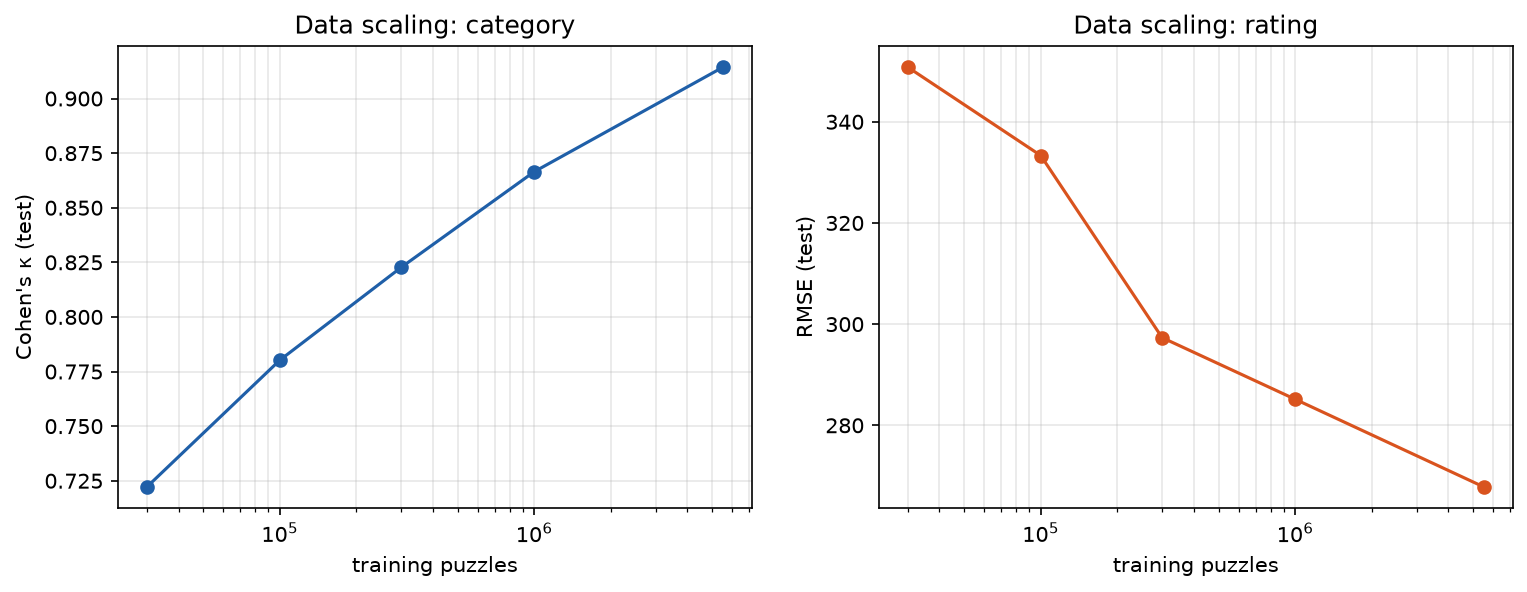
\includegraphics[width=\linewidth]{figures/nn_data_scaling.png}
\caption{Data scaling. Both heads keep improving to the full 5.5M puzzles; the curve has not flattened, so the model is limited by data rather than by capacity.}\label{fig:nn-scaling}
\end{figure}

Two results are negative and worth stating plainly. First, \textbf{multi-task learning does not help
either task here}: the category head alone reaches $\kappa = 0.870$ against $0.867$ when it shares a
trunk with themes and difficulty, and the difficulty head alone reaches RMSE 280 against 285. The
shared trunk costs a little on each task; what it buys is one model, one encoding pass and one file
instead of two, which is why the deployed model keeps it. Second, \textbf{the $\beta$-NLL correction
is not doing much work}. Plain noise-aware likelihood ($\beta = 0$) gives the best RMSE of the three
(283 against 285 at $\beta = 0.5$ and 289 at $\beta = 1$), and the differences are small either
way. The pathology that motivates
$\beta$-NLL~\cite{seitzer2022pitfalls} is that a learned variance can silence hard examples; here the
dominant part of the variance is the puzzle's \emph{known} rating deviation, and down-weighting a
noisily labelled puzzle is exactly the right thing to do, so the correction has little left to fix. On
another dataset without known label noise the argument for it would be stronger.
